% ****** Start of file apssamp.tex ******
%
%   This file is part of the APS files in the REVTeX 4.1 distribution.
%   Version 4.1r of REVTeX, August 2010
%
%   Copyright (c) 2009, 2010 The American Physical Society.
%
%   See the REVTeX 4 README file for restrictions and more information.
%
% TeX'ing this file requires that you have AMS-LaTeX 2.0 installed
% as well as the rest of the prerequisites for REVTeX 4.1
%
% See the REVTeX 4 README file
% It also requires running BibTeX. The commands are as follows:
%
%  1)  latex apssamp.tex
%  2)  bibtex apssamp
%  3)  latex apssamp.tex
%  4)  latex apssamp.tex
%
\documentclass[%
 reprint,
%superscriptaddress,
%groupedaddress,
%unsortedaddress,
%runinaddress,
%frontmatterverbose, 
%preprint,
%showpacs,preprintnumbers,
%nofootinbib,
%nobibnotes,
%bibnotes,
 amsmath,amssymb,
 aps,
%pra,
%prb,
%rmp,
prstab,
%prstper,
%floatfix,
]{revtex4-1}

\usepackage{graphicx}% Include figure files
\usepackage{dcolumn}% Align table columns on decimal point
\usepackage{bm}% bold math
%\usepackage{hyperref}% add hypertext capabilities
%\usepackage[mathlines]{lineno}% Enable numbering of text and display math
%\linenumbers\relax % Commence numbering lines
\usepackage{color}

%\usepackage[showframe,%Uncomment any one of the following lines to test 
%%scale=0.7, marginratio={1:1, 2:3}, ignoreall,% default settings
%%text={7in,10in},centering,
%%margin=1.5in,
%%total={6.5in,8.75in}, top=1.2in, left=0.9in, includefoot,
%%height=10in,a5paper,hmargin={3cm,0.8in},
%]{geometry}

\begin{document}

\title{Effects of pulsed hollow electron lens operation on the beam core in HL-LHC: \\First experimental studies and simulations.}% Force line breaks with \\
\thanks{Fermilab is operated by Fermi Research Alliance, LLC under
	Contract No.~DE-AC02-07CH11359 with the United States Department of
	Energy. This work was partially supported by the US DOE LHC
	Accelerator Research Program (LARP) and by the European FP7 HiLumi
	LHC Design Study, Grant Agreement 284404.}

\author{Miriam Fitterer}
 \email{mfittere@fnal.gov}
\author{Giulio Stancari}%
\author{Alexander Valishev}%
\affiliation{Fermi National Accelerator Laboratory, Batavia, Illinois, USA
% This line break forced with \textbackslash\textbackslash
}%

\author{Giulia Papotti}
\author{Stefano Redaelli}
\author{Daniel Valuch}
\affiliation{CERN, Geneva, Switzerland}%

\date{\today}% It is always \today, today,
             %  but any date may be explicitly specified

\begin{abstract}
In the HL-LHC a considerable amount of energy is stored in the beam tails due to the high beam intensity and an overpopulation of the tails compared to a Gaussian distribution. To control and clean the tail population, the installation of two hollow electron lenses, one per beam, is considered. Beside the DC operation, also a pulsed operation of the hollow electron lens is considered, which would considerably increase the diffusion speed by putting noise on the halo particles. In the ideal case, that is in case of no field at the beam core, only the halo particles are excited while leaving the core unperturbed. The picture though changes, if a residual field is present also at the location of the beam core putting noise also on the beam core. In this paper we present for estimates of the residual field at the beam core expected from the HL-LHC hollow electron lens and first experimental results of the effect of this excitation on the beam core together with the supporting simulations.
\end{abstract}

% PACS 2008:
% 29.20.db Storage rings and colliders

\pacs{29.20.D-}% PACS, the Physics and Astrtheonomy
                             % Classification Scheme.
%\keywords{Suggested keywords}%Use showkeys class option if keyword
                              %display desired
\maketitle

%\tableofcontents

\section{\label{sec:intro}Introduction}%force line break with \protect\\
Considering past, current and future high energy and intensity colliders, each new machine has represented a considerable leap in stored beam energy with rising values for future accelerators and colliders (see Table~\ref{tab:stored_energy}). 
\begin{table*}
	\caption{\label{tab:stored_energy}%
		Stored beam energy for different past, present and future colliders. Each new machine represents a leap in stored beam energy.
	}
	\begin{ruledtabular}
		\begin{tabular}{lccccc}
			Collider& Tevatron (protons) \cite{tevatron} & LHC 2016 \cite{} \footnote{values from \url{https://lhc-commissioning.web.cern.ch/lhc-commissioning/performance/2016-performance.htm}}& LHC nominal \cite{lhc_design} & HL-LHC \cite{} \footnote{values from parameter and layout committee website \url{https://espace.cern.ch/HiLumi/PLC/default.aspx}}& FCC \cite{fcc_param_2017} \footnote{get right reference and values}\\
			\colrule
			Beam energy [TeV] & 0.98 & 6.5 & 7.0 & 7.0 & 50.0\\
			Number of bunches & 36 & 2076 & 2808 & 2748 & ? \\
			Number of particles per bunch & $2.90\times 10^{11}$ & $1.18\times 10^{11}$ & $1.15\times 10^{11}$ & $2.2\times 10^{11}$ & $1.0\times 10^{11}$\\
			Stored beam energy [MJ] & 1.6 & 255.1 & 362.2 & 678.0 & 8400 \\
		\end{tabular}
	\end{ruledtabular}
\end{table*}
Recent measurements at the LHC furthermore show that the tails of the transverse beam distribution are overpopulated compared to a Gaussian distribution resulting in a considerable amount of energy being stored in the beam tails alone. In case of the LHC explicitly around 5\% of the beam population is stored in the tails above 3.5~$\sigma$ compared to 0.22\% in case of a Gaussian distribution leading to 19~MJ of stored energy in the tails in case of nominal LHC parameters and 34~MJ in case of HL-LHC~\cite{helreview_valentino}.

All of the above reasons lead to the conclusion that a mechanism is needed to deplete the beam tails in a controlled manner (see for example \cite{helreview} in case of HL-LHC). The most obvious idea is to decrease the collimator gaps or scrape the tails with a collimator type device \textcolor{red}{Why is that not possible?}. This is however not possible due to impedance issues. Other mechanisms must therefore be found to actively deplete the tails. Most promising are methods, which considerably increase the diffusion speed in the region of the tail particles while leaving the beam core unperturbed. The diffusing tail particles are then intercepted by the collimation system and removed (see FIG.~\ref{fig:active_halo_control} for illustration).
\begin{figure}[h]
	\begin{minipage}[t]{0.49\linewidth}
		\centering
		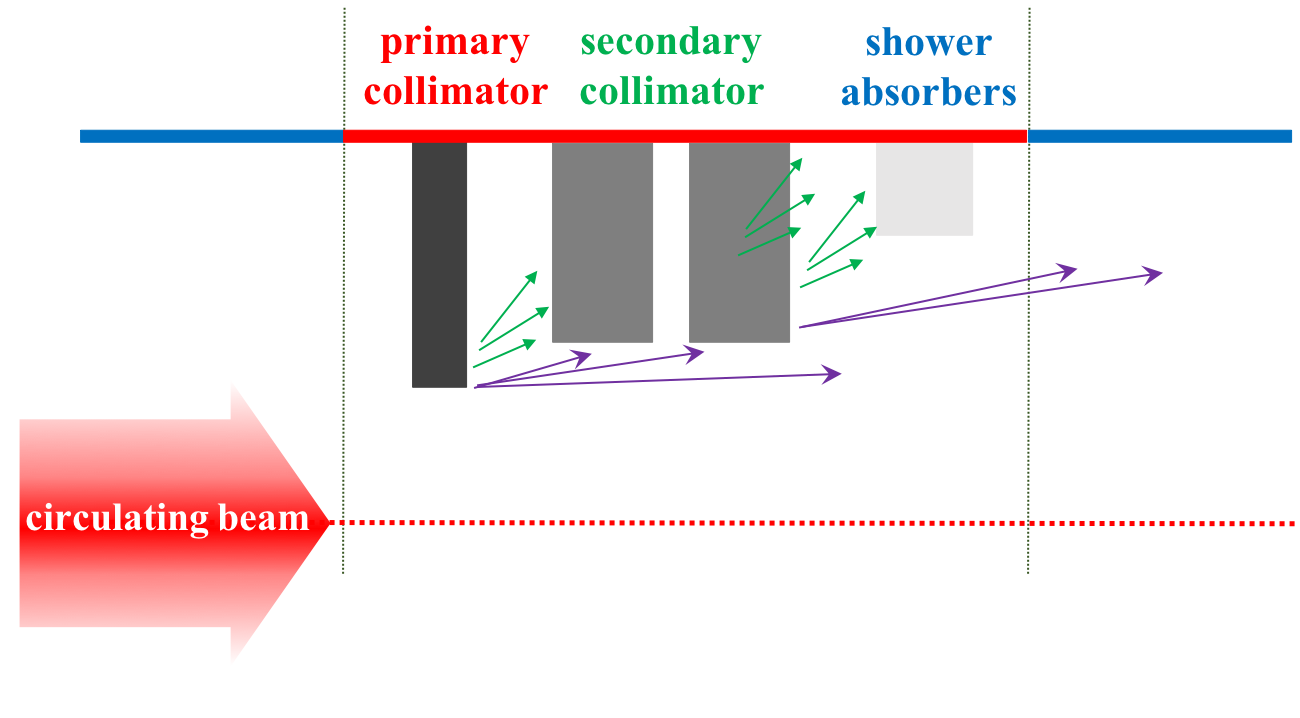
\includegraphics[width=1.0\linewidth]{passive_halo_control.png}
	\end{minipage}
	\begin{minipage}[t]{0.49\linewidth}
		\centering
		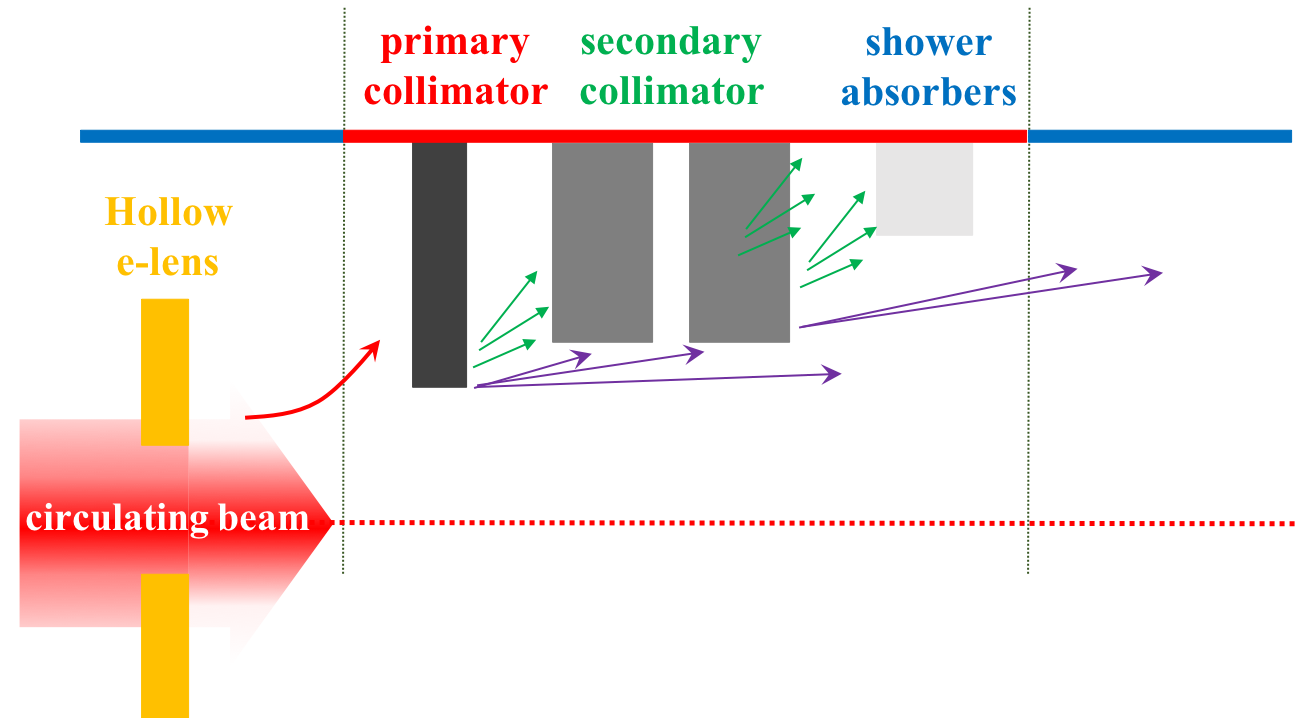
\includegraphics[width=1.0\linewidth]{active_halo_control.png}
	\end{minipage}	
	\caption{\label{fig:active_halo_control} Sketch of passive halo control as with the collimation system (top) and active halo control using in addition for example a hollow electron lens (HEL) to control the diffusion speed in the region tail region without affected the beam core (bottom). \textbf{Any acknowledgement needed for the plots?}.}
\end{figure}
In view of the need for LHC and HL-LHC in particular and in general for future high power accelerators, different methods have been studied in the last recent years \cite{helreview_bruce}, of which the HEL is considered the superior device at least in case of the HL-LHC \cite{helreview} and is also considered for other future high energy colliders like HE-LHC and FCC-hh \cite{,}.

The concept of active halo control however breaks down if also the beam core is affected, which would ultimately lead to a degradation of the performance. In this paper, we will concentrate on this aspect for the HEL foreseen to be installed in the HL-LHC. We will summarize possible sources of perturbations of the beam core concentrating in particular on the case of pulsed operation and with the focus on the beam experiments at the LHC performed in the context of these studies. 

This paper is structured as follows: Section~\ref{sec:hel} gives an introduction to the concept of HELs and summarizes the design parameters of the HL-LHC HEL. Section~\ref{sec:core} is dedicated to describing the sources of a residual field from the HEL in the core region. Section~\ref{sec:exp} presents the results of the LHC experiment to study the effects on the beam core in case of a pulsed operation of the HEL, explicitly a resonant excitation. This includes the detailed analysis of the observed losses, emittance and transverse beam distribution changes. To the knowledge of the authors, the observed distribution changes presented in this paper have never been measured before in the context of a resonant excitation. A resonant excitation has been previously studied at the Tevatron in the context of the HEL experiments \cite{hel_tevatron_stancari} and the abort gap cleaning used in operation \cite{hel_tevatron_abortgap_zhang}. Both studies however only concentrated on the losses and emittance changes without measuring the detailed changes of the distribution. In addition the presented experiment also provides scaling of the losses and emittance growth with the excitation amplitude allowing for a comparison with simulations and ultimately an extrapolation to HL-LHC.

\section{\label{sec:hel}Hollow electron lens for HL-LHC}
\begin{figure}[h]
	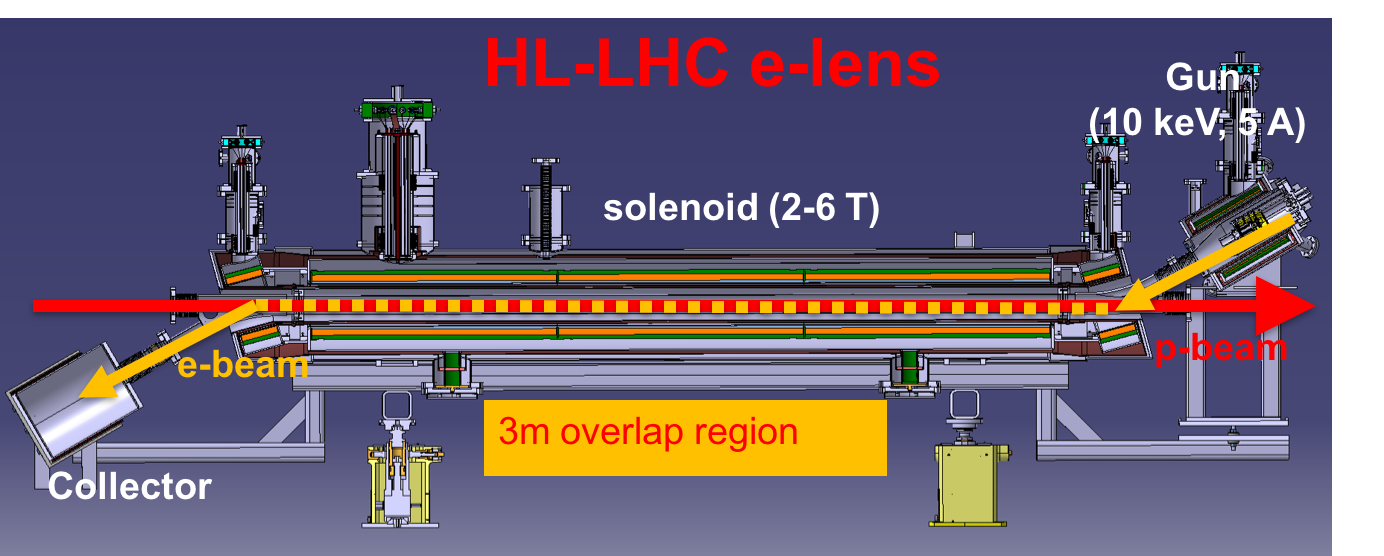
\includegraphics[width=1.0\linewidth]{hel_layout}% Here is how to import EPS art
	\caption{\label{fig:hel_layout} Layout of HL-LHC HEL \textbf{Ask Diego how to acknowledge correctly}.}
\end{figure}

\section{\label{sec:core}Sources of residual field in the proton beam core region}


\section{\label{sec:exp}LHC experiment}

\begin{acknowledgments}
We wish to acknowledge the support of the author community in using
REV\TeX{}, offering suggestions and encouragement, testing new versions,
\dots.
\end{acknowledgments}

\appendix

\section{Appendixes}


\bibliography{bibliography}% Produces the bibliography via BibTeX.

\end{document}
%
% ****** End of file apssamp.tex ******
